\section{ПОСТАНОВКА ЗАДАЧИ}

Имеются данные о спросе на некоторый товар за 4 года,
приведенные в таблице~\ref{tbl:source_data}.

\begin{table} [h!]
  \caption{
    Исходные данные
  }\label{tbl:source_data}
    \begin{tabular}{| m{11.4cm} | c |}
      \hline
      Период & Фактический спрос \\ \hline

      2008 кв. 1 & 19 \\ \hline
      2008 кв. 2 & 23 \\ \hline
      2008 кв. 3 & 27 \\ \hline
      2008 кв. 4 & 24 \\ \hline

      2009 кв. 1 & 18 \\ \hline
      2009 кв. 2 & 23 \\ \hline
      2009 кв. 3 & 31 \\ \hline
      2009 кв. 4 & 24 \\ \hline

      2010 кв. 1 & 21 \\ \hline
      2010 кв. 2 & 25 \\ \hline
      2010 кв. 3 & 33 \\ \hline
      2010 кв. 4 & 26 \\ \hline

      2011 кв. 1 & 22 \\ \hline
      2011 кв. 2 & 27 \\ \hline
      2011 кв. 3 & 26 \\ \hline
      2011 кв. 4 & 25 \\ \hline
    \end{tabular}
\end{table}

Как видно из графика, приведенного на рисунке~\ref{fig:source_data}, есть основания считать,
что спрос имеет сезонный характер.

\newpage

\begin{figure}[h!]
  \centering
  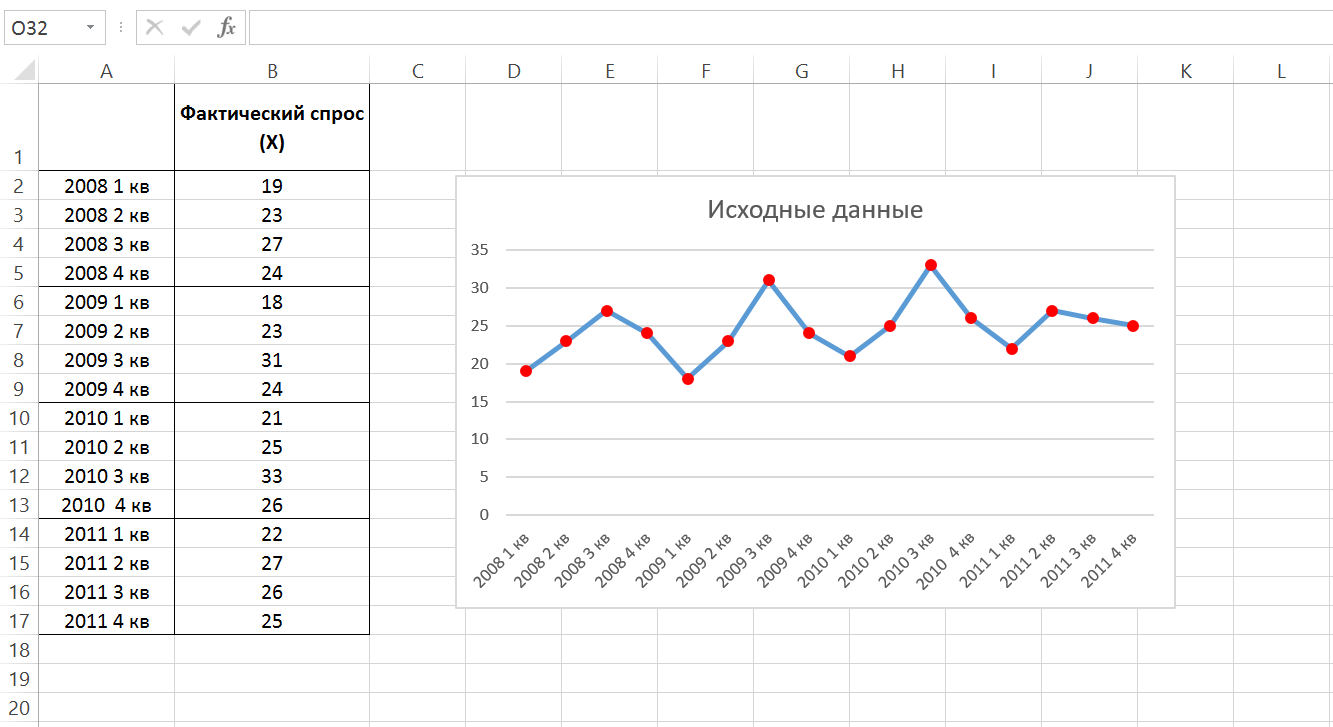
\includegraphics[width=160mm]{pic/source_data}
  \caption{Изменение анализируемой величины во времени}
  \label{fig:source_data}
\end{figure}

Требуется построить модели спроса с учетом сезонности:
\begin{itemize}
\item мультипликативная модель:
  \begin{equation*}
    \hat{x} = (a_0 + a_1t)*K_c,
  \end{equation*}
  \hspace{1.5mm} где \( \hat{x} \) --- прогнозируемая величина (спрос), \par
  \( a_0 \) и \( a_1 \) --- коэффициенты модели (их требуется определить), \par
  \( t \) --- номер периода, \par
  \( Kc \) --- коэффициенты сезонности (их также требуется определить);
\item аддитивная модель:
  \begin{equation*}
    \hat{x} = (a_0 + a_1t)+A_c,
  \end{equation*}
  \hspace{1.5mm} где \( A_c \) --- сезонная компонента.
\end{itemize}

Используя модели, найти прогноз на четыре квартала 2012 года.
Из этих моделей требуется выбрать наиболее точную.
